
\documentclass[a4paper,12pt]{article}
\usepackage{graphicx}
\usepackage{tikz}
\usepackage{hyperref}
\usetikzlibrary{shapes.geometric, arrows}

\tikzstyle{startstop} = [rectangle, rounded corners, minimum width=3cm, minimum height=1cm,text centered, draw=black, fill=red!30]
\tikzstyle{process} = [rectangle, minimum width=3cm, minimum height=1cm, text centered, draw=black, fill=blue!30]
\tikzstyle{arrow} = [thick,->,>=stealth]

\title{Practical Work 1: TCP File Transfer}
\author{Phạm Phú Hưng}
\date{\today}

\begin{document}

\maketitle

\section*{Overview}
This practical work aims to implement a 1-to-1 TCP file transfer system using socket programming. The setup includes:
\begin{itemize}
    \item One server to handle file transfers
    \item One client to request and receive the file
    \item Communication over TCP/IP
\end{itemize}

The following sections explain the protocol design, system organization, implementation, and team responsibilities.

\section*{Design Protocol}
The file transfer protocol follows these sequential steps:
\begin{enumerate}
    \item The \textbf{server} initializes and binds a socket to an address and port.
    \item The server listens for incoming \textbf{client connections}.
    \item The \textbf{client} initiates a connection request to the server.
    \item Once connected, the client requests a file, and the server sends the file in chunks.
    \item After completion, both the client and server close the connection.
\end{enumerate}

The following diagram illustrates the protocol:

\begin{figure}[h]
    \centering
    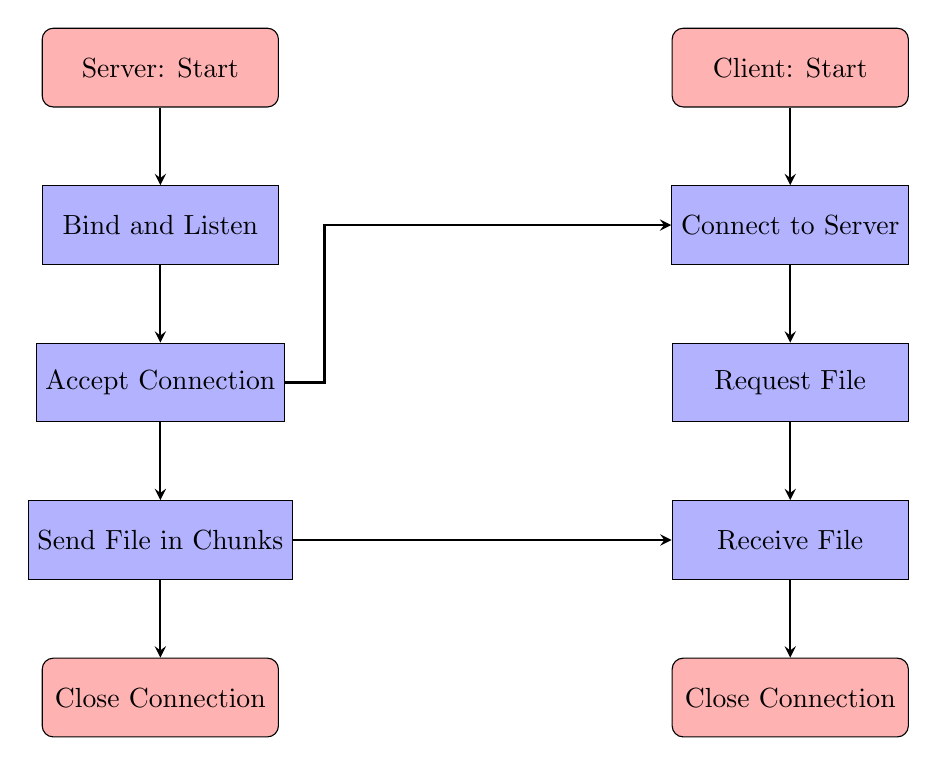
\begin{tikzpicture}[node distance=2cm]

    % Nodes
    \node (start) [startstop] {Server: Start};
    \node (bind) [process, below of=start] {Bind and Listen};
    \node (accept) [process, below of=bind] {Accept Connection};
    \node (read) [process, below of=accept] {Send File in Chunks};
    \node (close) [startstop, below of=read] {Close Connection};

    % Arrows for Server
    \draw [arrow] (start) -- (bind);
    \draw [arrow] (bind) -- (accept);
    \draw [arrow] (accept) -- (read);
    \draw [arrow] (read) -- (close);

    % Client side
    \node (start_client) [startstop, right of=start, xshift=6cm] {Client: Start};
    \node (connect) [process, below of=start_client] {Connect to Server};
    \node (request) [process, below of=connect] {Request File};
    \node (receive) [process, below of=request] {Receive File};
    \node (close_client) [startstop, below of=receive] {Close Connection};

    % Arrows for Client
    \draw [arrow] (start_client) -- (connect);
    \draw [arrow] (connect) -- (request);
    \draw [arrow] (request) -- (receive);
    \draw [arrow] (receive) -- (close_client);

    % Connection Arrows
    \draw [arrow] (accept.east) -- ++(0.5,0) |- (connect.west);
    \draw [arrow] (read.east) -- ++(0.5,0) |- (receive.west);

    \end{tikzpicture}
    \caption{Protocol Design for File Transfer}
    \label{fig:protocol}
\end{figure}

\section*{System Organization}
The system is organized using a client-server architecture. The following diagram shows the structure of the system:

\begin{figure}[h]
    \centering
    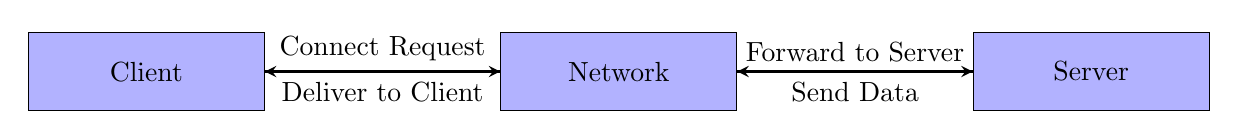
\begin{tikzpicture}[node distance=2cm]

    % Nodes
    \node (client) [process] {Client};
    \node (network) [process, right of=client, xshift=4cm] {Network};
    \node (server) [process, right of=network, xshift=4cm] {Server};

    % Arrows
    \draw [arrow] (client.east) -- node[anchor=south] {Connect Request} (network.west);
    \draw [arrow] (network.east) -- node[anchor=south] {Forward to Server} (server.west);
    \draw [arrow] (server.west) -- node[anchor=north] {Send Data} (network.east);
    \draw [arrow] (network.west) -- node[anchor=north] {Deliver to Client} (client.east);

    \end{tikzpicture}
    \caption{System Organization: Client-Server Architecture}
    \label{fig:system}
\end{figure}

\section*{Implementation}
The file transfer is implemented using Python socket programming. Below are snippets for the server and client implementations.

\subsection*{Server Code}
\begin{verbatim}
# Python example
import socket

server_socket = socket.socket(socket.AF_INET, socket.SOCK_STREAM)
server_socket.bind(('0.0.0.0', 8080))
server_socket.listen(1)

conn, addr = server_socket.accept()
print(f"Connection from {addr}")
with open('file.txt', 'rb') as file:
    conn.sendfile(file)
conn.close()
server_socket.close()
\end{verbatim}

\subsection*{Client Code}
\begin{verbatim}
# Python example
import socket

client_socket = socket.socket(socket.AF_INET, socket.SOCK_STREAM)
client_socket.connect(('server_ip', 8080))

with open('received_file.txt', 'wb') as file:
    data = client_socket.recv(1024)
    while data:
        file.write(data)
        data = client_socket.recv(1024)
client_socket.close()
\end{verbatim}

\section*{Roles and Contributions}
\begin{itemize}
    \item \textbf{Phạm Phú Hưng:} Designed the protocol and implemented the server code.
    \item \textbf{Team Member 2:} Developed the client code and tested the system.
    \item \textbf{Team Member 3:} Verified the error handling and documented the project.
\end{itemize}

\section*{Conclusion}
The project successfully demonstrates a reliable 1-to-1 TCP file transfer system using Python sockets. The implemented protocol ensures robust error handling and orderly connection management.

\end{document}
